% !TEX root =../thesis.tex
\chapter{Introduction}
\label{chap:intro}

\lettrine[lines=4]{F}{or} millenia mankind has watched and studied the nightsky. Apart from planets and comets it appeared an immuatble canvas on which the stars rested. It comes as no surprise that for ancient civilizations supernovae (which were very rare events, occuring only every few centuries ) were interpreted as important Omens as they broke the paradigm of the unchanging nightskies. As these events are so rare their origin remained a mystery until the middle of the last century \citet{1934PNAS...20..254B} suggested that "the phenomenon of a super-nova represents the transition of an ordinary star into a body of considerably smaller mass". For the last 85 years the "supernova-branch" in astronomy has been developing. There have been many advances, but there are still very unknowns about supernovae. This work addresses two subfields of supernovae: The unsolved progenitor problem for Type Ia Supernovae as well as quantifying the nucleosynthetic yield of Type Ia supernovae from low-resolution spectra.


\section{Ancient Supernovae}
\label{sec:ancientsn}

One of the earliest recorded supernovae is SN185. It first appeared in December of 185 and was visible (however fading) till the August of 187. The main record is the \textit{Houhanshu} \citep{2006ChJAA...6..635Z} which had a described it to be close to $\alpha$ \textit{cen}. Follow-up in modern times have revealed a supernova remnant in a distance of roughly 1\;kpc near the $\alpha$ \textit{cen} \citep{2006ChJAA...6..635Z}. SN185 is often named as the oldest written record of a supernova, this is however sometimes contested as it is still not completely clear if the so called "guest star" was a comet or a supernovae. 

The oldest undisputed record of a supernova is SN1006. It was observed worldwide by asian, arabic and european astronomers. 
mention 1885 in andromeda\cite{1885AN....112..360H}


\section{Modern supernova observations and surveys}
\label{sec:}
The most famous and often quoted paper is \citet{1934PNAS...20..254B}. It termed the term supernova and established the difference between common novae and supernovae. \citet{1934PNAS...20..254B} suggested that these luminous events are caused by the death of stars. 

In order to understand the phenomenon of the supernova better Zwicky began a supernova search with the 18-inch Schmidt telescope. He found several supernovae cite?? which in turn inspired Minkowski to classify these supernovae by their spectra \citet{1941PASP...53..224M}. 
He categorized the 14 known objects into two categories. Those without hydrogen he called 'Type I', those with hydrogen he called 'Type II' (see section \ref{sec:sn_classification} for a more detailed description).

With the advent of affordable computing in the 1960s the first computer controlled telescopes were build. The 24-inch telecope was built by the Northwestern University and was deployed in Corralitos Observatory in New Mexico. This search resulted 14 supernovae. 

The 1990's can be described as the decade of the supernova surveys. The Leuschner Observatory Supernova Survey began in 1992 followed shortly by the Berkeley Automatic Imaging Telescope (BAIT). These searches resulted in 15 supernovae by 1994 \citep{1994AAS...185.7905V}. One of the most well known discoveries is SN 1994D. This supernovae was observed with the Hubble Space Telescope and resulted in an image that is widely used today (see Figure \ref{fig:sn1994d}).

These successful programmes were succeeded by the Lick Observatory Supernova Search (LOSS) using the Katzman Automatic Imaging Telescope (KAIT). By the year 2000 it had found 96 supernovae \citep{2001ASPC..246..121F}.


\section{Supernova classification}
\quote{Gallia est omnis divisa in partes tres.}

\label{sec:sn_classification}
The classification of supernovae started in the 1941 when Minkowski realized that there seem to be two main types \citep{1941PASP...53..224M}. Minkowski relied on optical low-resolution spectra near the maximum to identify the two main subtypes (see Figure \ref{fig:sn_spectra_turatto} for an overview of spectra of different types). Those containing a hydrogen line (6563 \AA) he called Type II supernovae and those showing no hydrogen he called Type I supernovae.  

\begin{figure}[htbp] %  figure placement: here, top, bottom, or page
   \centering
   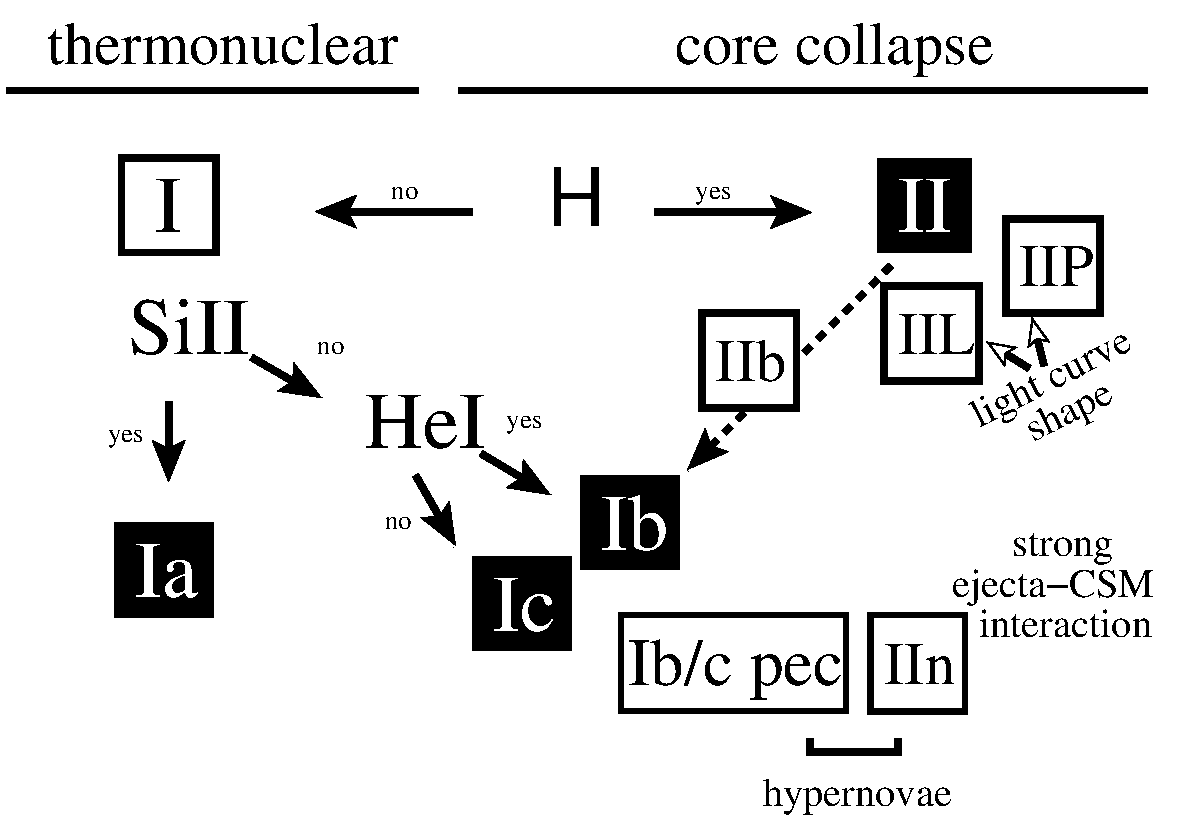
\includegraphics[width=\textwidth]{chapter1/plots/sn_classification.pdf} 
   \caption{}
   \label{fig:sn_classification}
\end{figure}

This basic classification has remained to this day, however the two main classes branched into several subtypes.
During the 1980s the community discovered that most \sneia\ showed a broad Si II line at 6130 \AA, but that there was a distinct subclass of objects that lacked this feature. These Silicon-less objects were then subclassed further into objects that showed helium -- now known as Type Ib --  and those that did not were called Type Ic \citep{1987ApJ...317..355H, 1986ApJ...306L..77G}. The classical Type I supernova was renamed to Type Ia (see Figure \ref{fig:sn_classification}). 

\begin{figure}[htbp] %  figure placement: here, top, bottom, or page
   \centering
   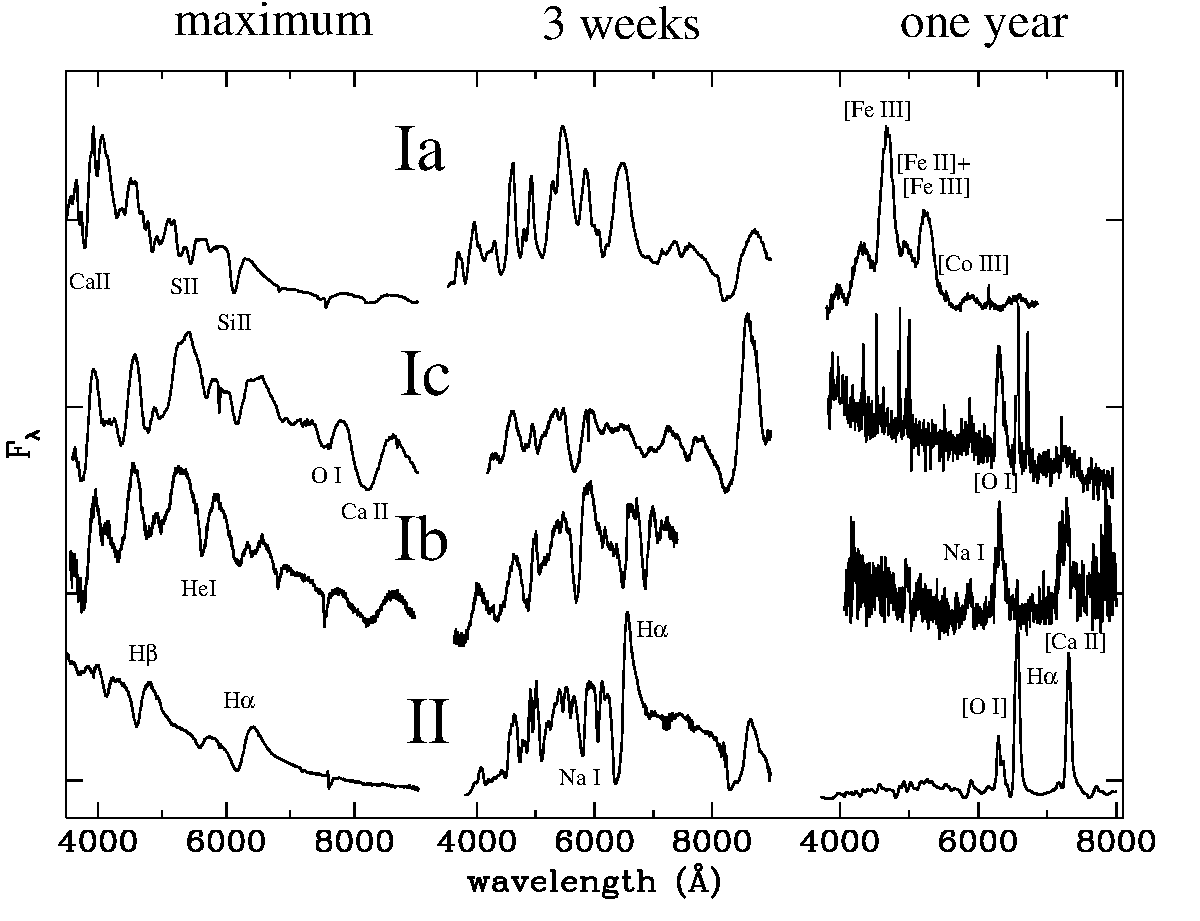
\includegraphics[width=\textwidth]{chapter1/plots/sn_class_spectra.pdf} 
   \caption{example caption}
   \label{fig:sn_class_spectra}
\end{figure}

This classification only uses static spectral features. In recent years, however, there has been a push towards also using the lightcurve and spectral evolution as classification parameters. \citet{2005ApJ...623.1011B} provide an overview of this subclassing of \sneia\ and suggest that there are two distinct subclasses of \sneia. As a parameter for this further partitioning they use the velocity measured from the Si II feature at 6355 \AA. Those with a relatively fast decline in this radial velocity they call \hvg\ (high velocity gradient) those with a slow decline rate are named \lvg\ (low velocity gradient). 
Figure \ref{fig:sn_class_lvg_hvg} shows the velocity gradient of 26 supernovae taken from  \citet{2005ApJ...623.1011B}

\begin{figure}[htbp] %  figure placement: here, top, bottom, or page
   \centering
   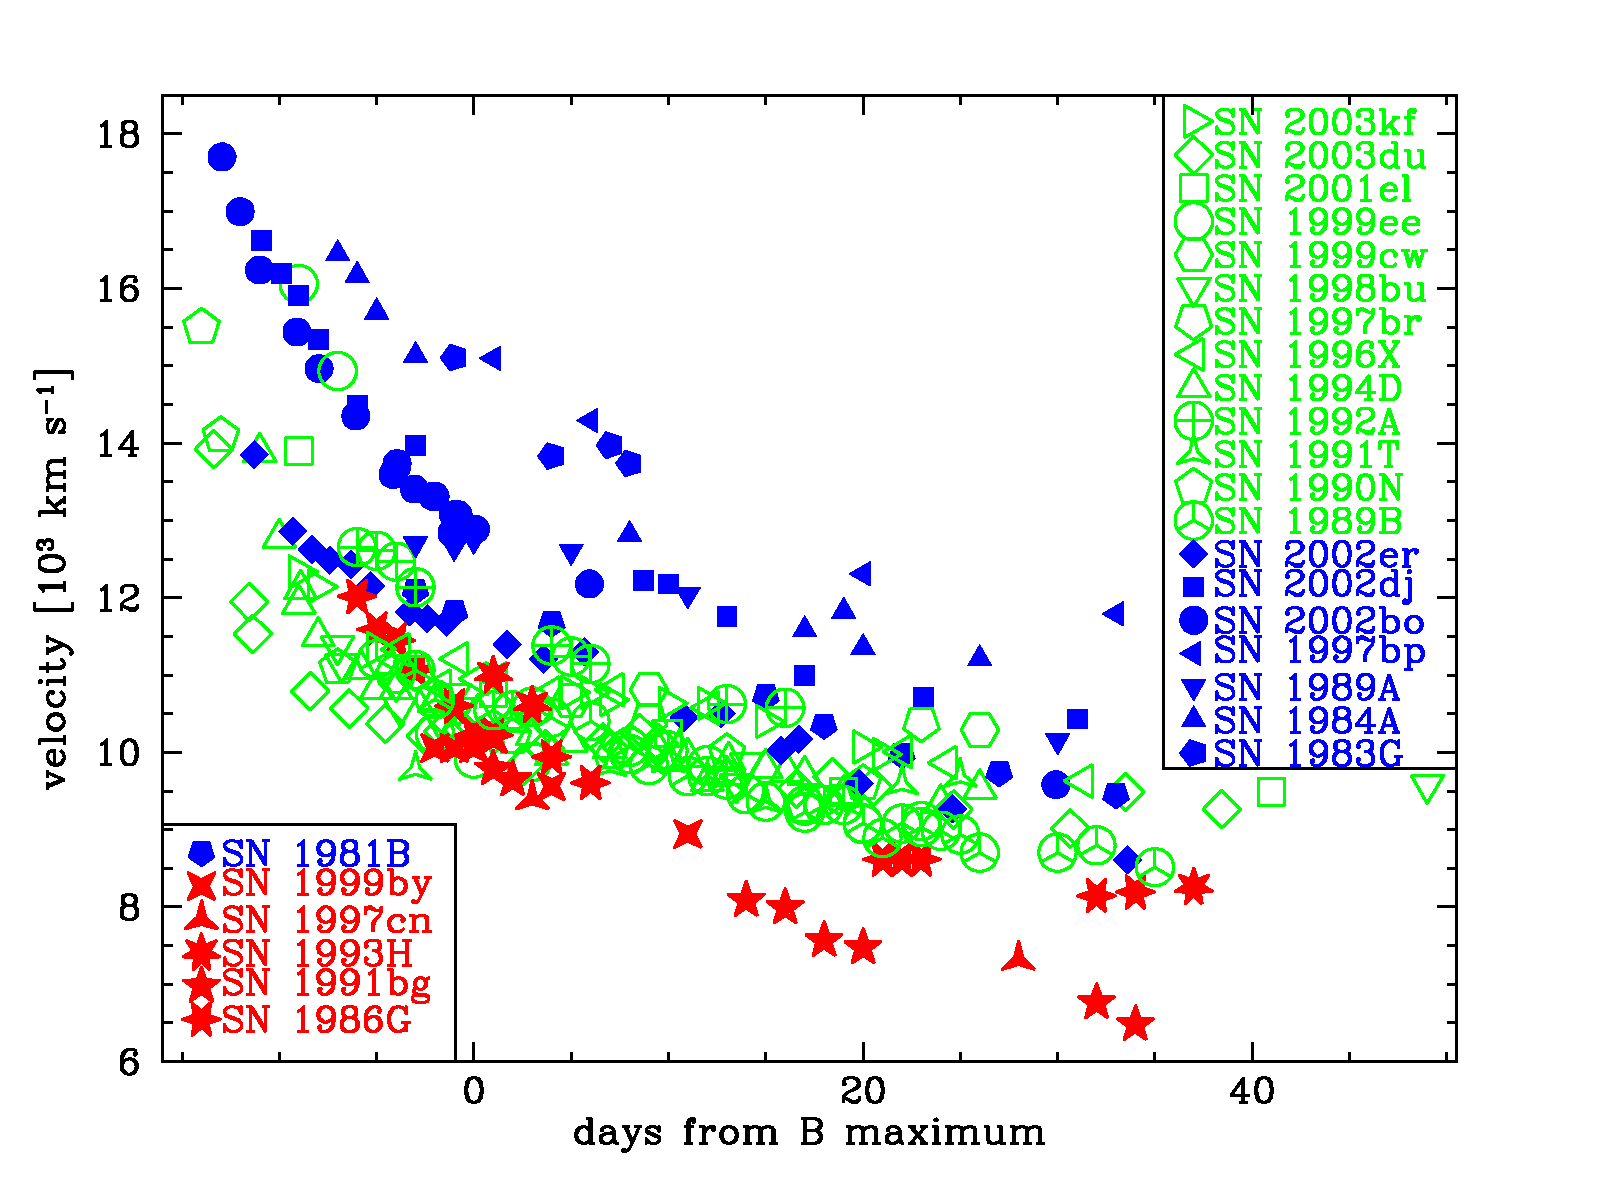
\includegraphics[width=\textwidth]{chapter1/plots/velocity_gradient.pdf} 
   \caption{example caption}
   \label{fig:sn_class_lvg_hvg}
\end{figure}

Futhermore there seems to be also a split in the intrinsic luminosity of \sneia. The canonical objects for these distinct brightness classes are the overluminous 1991T \citet{1992AJ....103.1632P} and the faint 1991bg .
Faint supernovae are fast decliners both in velocity as well as luminosity \citet{2005ApJ...623.1011B}. The bright supernovae seem to occur in both the \hvg\ and \lvg\ group. I will discuss the physical implications of these two subtypes in section \ref{sec:snia_physics}.

In summary, although there are several different subclasses the \snia as a class itself is relatively homogenous when compared to the different \sneii. ??? rates????


\sneii span large ranges in observables like luminosity, explosion energies, etc. We can divide the main class into three main subclasses Type II Plateau \citet[\sniip][]{1979A&A....72..287B} which have a relatively flat lightcurve after an initial maximum, in contrast the Type II Linear \cite[\sniil][]{1990MNRAS.244..269S} has a rapid linear decline after the maximum. The third subclass is the narrow-lined \snii (\sniin) which is characterized by narrow emission lines, which are thought to come from interaction with the \csm. Unlike the \sneia there are numerous intermediate objects among these three basic classes. 

???? 

For a more comprehensive review of the classification of supernovae the reader should consult \citet{2003LNP...598...21T, 2007AIPC..937..187T}.

\section{Type II Supernova}
\subsection{Observation}

\subsection{Theory}


nucelosynthesis
first stars
hypernovae
GRB connection
massive stars
expanding photosphere -> distance measurements
binary evoltion

\section{Type Ib/c Supernova}


\section{Type Ia Supernova}
binary evolution
chandrasekhar
white dwarfs
nucleosynthesis
iron in particular

cosmology

\section{Progenitors of Type Ia progenitors}
\label{sec:snia_progenitor}


